%\documentclass[a4paper]{article}
\documentclass[12pt]{article}
%% Language and font encodings
\usepackage[english]{babel}
\usepackage[utf8x]{inputenc}
\usepackage[T1]{fontenc}
\usepackage{multicol}
%% Sets page size and margins
\usepackage[a4paper,top=3cm,bottom=2cm,left=3cm,right=3cm,marginparwidth=1.75cm]{geometry}
\usepackage{fancyhdr}
\usepackage{soul}
%\usepackage{hyperref}
\usepackage{threeparttable}


%% Useful packages
\usepackage{amsmath}
\usepackage{graphicx}
\usepackage[colorinlistoftodos]{todonotes}
\usepackage[colorlinks=true, allcolors=blue]{hyperref}
%\AtBeginDocument{\renewcommand{\bibname}{References}}
\pagestyle{fancy}
\fancyhf{}
\rhead{$\textrm{SM}^2$}
\lhead{NEMD Workshop}
\rfoot{\thepage}

\title{Report}
\author{}
\date{\today}

\begin{document}
%\maketitle
\begin{titlepage}
        \centering
        {\scshape\Large\bfseries Non-equilibrium molecular dynamics workshop \par} 
        \vfill
        {\Large\bfseries LAMMPS Hands-on Session \par}
        \vfill
        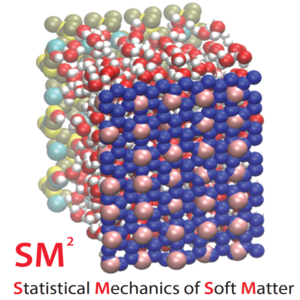
\includegraphics[width=0.5\textwidth]{sm2_logo.png}\par %\vspace{5cm}
        \vfill

\end{titlepage}

\newpage
\tableofcontents
\newpage

\section{Running an MD simulation}
To run a molecular dynamics (MD) simulation using 
Large-scale Atomic/Molecular Massively Parallel Simulator (LAMMPS) we generally need two files.
The first file is called a LAMMPS input script which consists of the commands required to run
a MD simulation.
The second file called the system file contains the description of the system, atom coordinates, bonds, system size, etc. and is read by the LAMMPS script at the start of a simulation.
In some cases the system can be created in the LAMMPS script itself and in such cases we 
require only the LAMMPS input script to run the simulation.
A general outline of a LAMMPS MD simulation is given below,

\begin{enumerate}
\centering
\item Setting up the system\\
(In this step either the system information is read by LAMMPS or 
the required system is created in the input script itself.)
$$\big\Downarrow$$
\item Providing interaction potentials \\
(In this step the atomic/molecular interaction information is provided to LAMMPS.
For complex or real systems we should refer the literature to obtain the 
appropriate values for interaction parameters.) \\
$$\big\Downarrow$$ 
\item System minimization \\
(In this step LAMMPS adjust the atom coordinates to attain a minimum potential energy state for 
the system. Though not necessary it is advisable to perform this step since it can prevent the 
system from blowing up due to bad intial system configuration.) \\
$$\big\Downarrow$$
\item Setting up the system temperature \\
(In this step LAMMPS will bring the system to the required temperature.
Different thermostatting schemes are available in LAMMPS to achieve the required temperature.) \\
$$\big\Downarrow$$
\item Running the system in the required ensemble and output \\
(In this step the system is allowed to evolve in the required statistical ensemble and 
output information is collected from LAMMPS for further analysis.)

\end{enumerate}

\newpage
\subsection{Some frequently used LAMMPS commands}
\begin{itemize}
\item atoms\_style $\Rightarrow$ To define the attributes of the simulation pariticles.
\item region $\Rightarrow$ To define a geometeric region which can be later accessed 
in the LAMMPS script.
\item group $\Rightarrow$ To identify a set of particles as a single group.
\item pair\_style, pair\_coeff $\Rightarrow$ To define the interaction parameters for the particles.
\item set $\Rightarrow$
\item fix $\Rightarrow$
\item compute $\Rightarrow$
\item dump, thermo\_style $\Rightarrow$
\end{itemize}

\newpage
\section{Atomic System}
\begin{itemize}
\item LAMMPS filename: atomic.lmp
\item Here we simulate an atomic system containing Lennard-Jones (LJ) particles with 
reduced density, $\rho^{*} = 0.8$.
\item The values for LJ interaction parameters $\sigma$ and $\epsilon$ are kept equal to 1.
\item The LJ interaction cutoff, $r_c$ is equal to $2.5\sigma$.
\item System dimensions: $10\sigma \times 10\sigma \times 10\sigma$ 
($L_{x} \times L_{y} \times L_{z}$).
\item System is equilibrated to a reduced temperature $T^{*} = 0.8$, 
using a Nos\'e-Hoover thermostat in LAMMPS.
\item The simulation outputs the radial distribution function (RDF) of the 
present atomic system.
\item The RDF values obtained from the simulation is compared with the RDF plot given 
in Page 70 of the book `Computer Simulation of Liquids' by Allen and Tildesley. 
\end{itemize}

%\newpage
\section{Poiseuille System}
\begin{itemize}
\item LAMMPS filename: poiseuille.lmp
\item Here we simulate a system where a fluid is confined between two walls.
\item All particles in the system are modelled as LJ particles.
\item The values for LJ interaction parameters $\sigma$ and $\epsilon$ between the fluid particles 
and between a fluid particle and a wall particle are kept equal to 1.
\item The walls are kept as rigid i.e., there is no interaction between wall particles.
\item The LJ interaction cutoff, $r_c = 2.5\sigma$
\item Channel width: $20\sigma \ (L_{z})$.
\item Wall area: $10\sigma \times 10\sigma \ (L_x \times L_y)$.
\item The system is equilibrated to a temperature, $T^* = 1.0$ by thermostating the fluid using a
Nos\'e-Hoover thermostat.
\item We apply an acceleration, $\vec{a} = 0.075\hat{i} + 0 \hat{j} + 0\hat{k}$ (LJ units) to 
every fluid particle in the system to simulate a Poiseuille flow.
\item The simulation outputs the velocity and density variation w.r.t the confined direction.
\end{itemize}

\newpage
\section{Water System}
\begin{itemize}
\item LAMMPS filename: water.lmp
\item Here we simulate a water box containing 256 SPC/E water molecules with 
density $1 \ \textrm{g} \ \textrm{cm}^{-3}$.
\item The values for interaction parameters is taken from 
`Mark, P., \& Nilsson, L. (2001). Structure and dynamics of the TIP3P, SPC, and SPC/E water models at 298 K. The Journal of Physical Chemistry A, 105(43), 9954-9960.'
\item Simulation box dimensions: $20 \times 20 \times 20 \ \textrm{\AA}^{3}$ 
($L_{x} \times L_{y} \times L_{z}$).
\item System is initially equilibrated to a temperature of 298 K and 1 bar pressure, 
using a Nos\'e-Hoover barostat in LAMMPS.
\item The simulation outputs RDF ($g_{H-H}(r)$, $g_{H-O}(r)$, and $g_{O-O}(r)$) and 
Mean square displacement (MSD) of the water system.
\item The Self-diffusion coefficient (D) is calculated from the MSD of all oxygen 
atoms using the Einstein relation,
$$\textrm{MSD} = \lim_{t\to\infty}\langle |\vec{r}(t^{*}+t) - \vec{r}(t^{*})|\rangle = 6Dt.$$
\end{itemize}

\section{SLLOD System}
\begin{itemize}
\item LAMMPS filename: sllod.lmp
\item Here we simulate an atomic system containing LJ particles with density, $\rho^{*} = 0.8$.
\item The values for LJ interaction parameters $\sigma$ and $\epsilon$ are kept equal to 1.
\item The LJ interaction cutoff, $r_c$ is equal to $2.5\sigma$.
\item Initial system dimensions: $10\sigma \times 10\sigma \times 10\sigma$ 
($L_{x} \times L_{y} \times L_{z}$).
\item Initially the system is equilibrated to a reduced temperature $T^{*} = 1.0$, 
using a Nos\'e-Hoover thermostat in LAMMPS.
\item After the initial equilibration an engineering strain rate, $\dot{\gamma}$ is 
applied to the system.
\item Since application of a strain rate will change the simulation box dimensions, we use 
\href{https://docs.lammps.org/fix_nvt_sllod.html}{nvt/sllod} thermostatting technique in LAMMPS
to thermostat the system.
\item The simulation outputs all the components of the pressure tensor of the system.
\item The shear viscosity ($\eta$) is calculated from the off-diagonal($xy$) element of the pressure tensor
as,
$$ \eta = -\frac{P_{xy}}{\dot{\gamma}}.$$

\end{itemize}

\appendix

\section{Appendix}
LAMMPS require C language and MPI protocol to be pre-installed, hence make sure that 
both of them are already installed in your system before running the simulation.
Data analysis and plotting will be done using Python language, hence it is recommended that you 
install python and some of its libraries (Numpy, Scipy and Matplotlib) to run the Python scripts.

\subsection{Installing LAMMPS}

\subsubsection{Linux Systems}
\$ sudo add-apt-repository ppa:gladky-anton/lammps\\
\$ sudo add-apt-repository ppa:openkim/latest\\
\$ sudo apt-get update\\
\$ sudo apt-get install lammps-daily\\

\subsection{Installing VMD}

Download the latest version of VMD for the corresponding OS from 
\href{https://www.ks.uiuc.edu/Development/Download/download.cgi?PackageName=VMD}{here} 
(You might need to create account with VMD inorder to download the package).
After downloading the package unzip the package and open the terminal in the 
go to the VMD package directory and enter the following commands,\\
\$ ./configure \\
\$ cd src \\ 
\$ sudo make install \\
\$ vmd \\

\subsection{Installing Packmol}




%\begin{figure}[h!]
%\begin{tabular}{cc}
%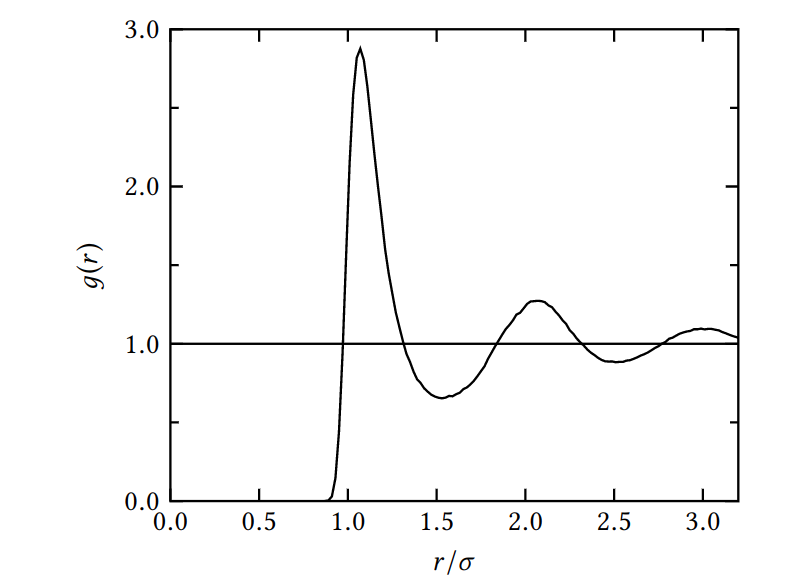
\includegraphics[width=0.5\textwidth]{./plots/allen_rdf.png} &
%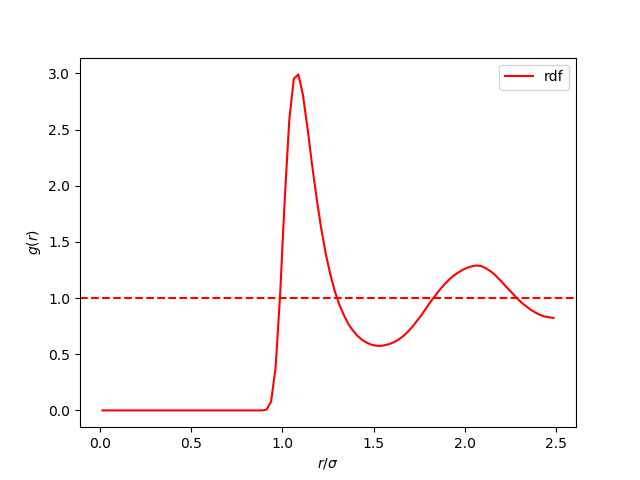
\includegraphics[height=0.4\textwidth, width=0.5\textwidth]{./plots/atomic_rdf.png}
%\end{tabular}
%\caption{\label{fig:1} }
%\end{figure}

%%%%%%%%%%%%%%%%%%%%%%%%%%%%%%%%%%%%%%%%%%%%%%%%%%%%%%%%%%%%%%%%%%%%%%%%%%%%%%

\end{document}
